\section{Results}

At the conclusion of the initial LUX science run, in December of 2013, a total of 10 Bq of tritium was injected into LUX and removed. A total 325,000 events were observed in the active volume of LUX. 183,000 events occurred in the fiducial volume at the nominal LUX electric field of 180 V/cm with about 4 of those being due to non-tritium energy deposits. Another set with 4,500 fiducial events was collected in a special run at a reduced field of 105 V/cm. The S1 and S2 signals are corrected for spatial effects such as the light collection efficiency and the free electron lifetime with $\rm ^{83m}$Kr data as described in \cite{lux-reanalysis} and in further detail in \cite{Dobi_Thesis}. 

For an electronic recoil (ER), the light and charge created result from excitation and ionization produced by the recoiling electron. Excitons and recombining electron ion pairs will each produce a single 175 nm photon, electrons that escape recombination are extracted at the expense of a single photon. We interpret the data in terms of the combined energy model for electron recoils \cite{Platzman}, where the total energy of an event is directly proportional to the number of quanta produced (electrons plus scintillation photons):

\begin{equation}
\begin{split}
\rm E_{total}= W \cdot (n_i + n_{ex}) \\
\rm E_{total} = W \cdot (n_{\gamma} + n_e )
\label{platzman_eq}
\end{split}
\end{equation}

\noindent
Where $\rm E_{total}$ is the energy of the deposition in keV and $\rm n_i$, $\rm n_{ex}$, $\rm n_\gamma$ and $\rm n_e$ are the number of ions, excitons, photons and electrons respectively.We use a $W$ value of 13.7 $\rm \pm$ 0.2 eV/quanta \cite{Dahl_Thesis}, as discussed in section \ref{sec:LXe_Theory}. In LUX $n_{\gamma}$ and $n_e$ are proportional to the S1 and S2 signals, with gain factors $g_1$ and $g_2$: 
%We use a $W$ value of 13.7 $\rm \pm$ 0.2 eV/quanta \cite{Dahl_Thesis}. In LUX $n_{\gamma}$ and $n_e$ are proportional to the S1 and S2 signals, with gain factors $g_1$ and $g_2$:

\begin{equation}
\rm E_{total} = W \cdot \left(\frac{S1}{g_1} + \frac{S2}{g_2} \right)
\label{energy_eq}
\end{equation}

\noindent
where S1 and S2 have units of photons detected (phd) and $g_1$ and $g_2$ have units of phd per quanta. $g_1$ is the average light collection efficiency times the average quantum efficiency of the PMT arrays, while $g_2$ is the product of the electron extraction efficiency at the liquid-gas surface and the average single electron size in phd. $g_1$ and $g_2$ were measured for the science run with line source data in LUX as described in Ref. \cite{lux-reanalysis, lux-prd}. For the December 2013 analysis presented in this paper the gains g1 and g2 are constrained by optimizing the combined energy model to the true tritium spectral shape \cite{Tritium_Eq_Simpson} convolved with detector resolution \cite{Dobi_Thesis}. We find values of $g_1$ = \gone and  $g_2$ = \gtwo, consistent with the values found for the science run.

\begin{figure}[h!]\centering
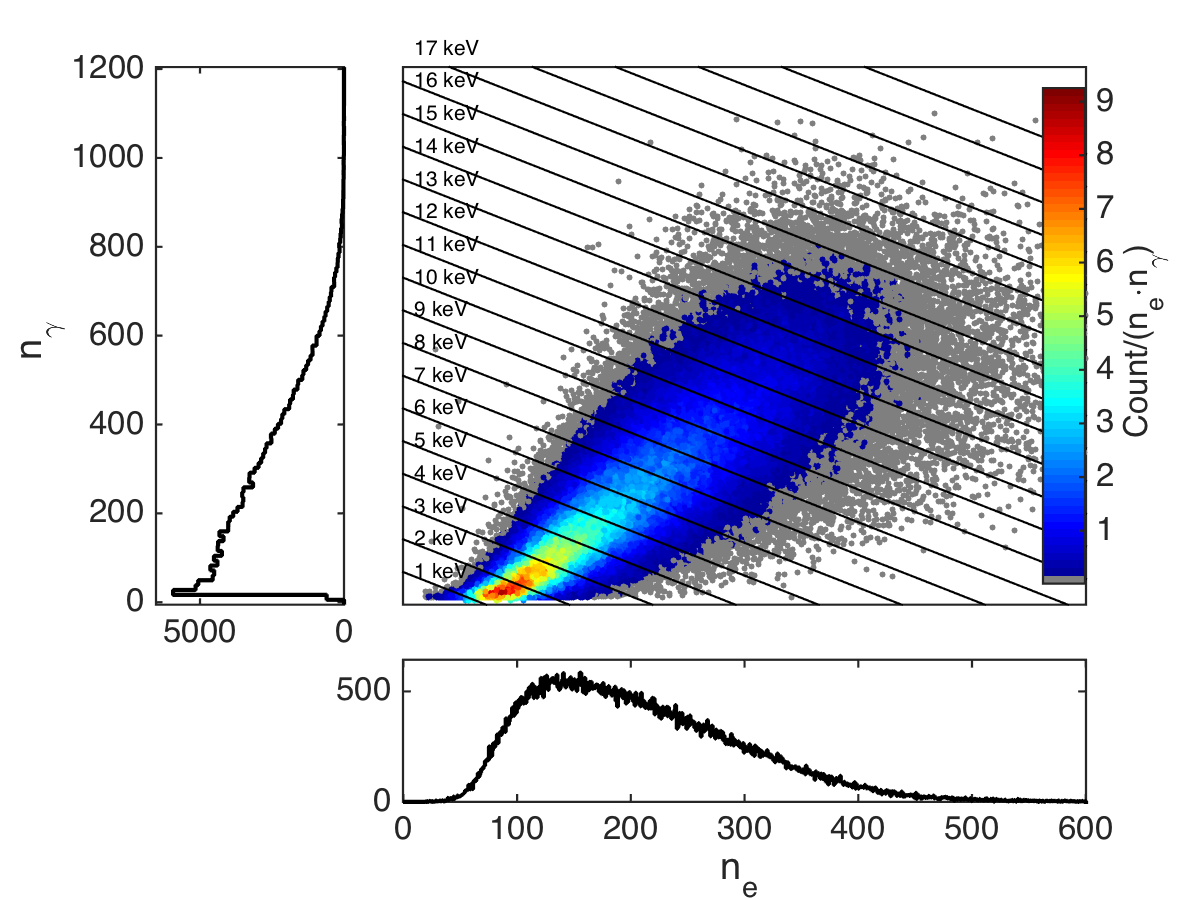
\includegraphics[width=90mm]{fig/tritium_scatter.png}
\caption{Scatter plot of $n_e$ vs $n_{\gamma}$ for 149,000 fiducial tritium events at 180 V/cm. Lines of constant energy are indicated assuming a $W$ value of 13.7 eV/quanta. The data is projected into $n_e$ and $n_{\gamma}$ histograms on each axis.}
\label{fig:tritium-scatter}
\end{figure}


\begin{figure}[h!]
\begin{center}
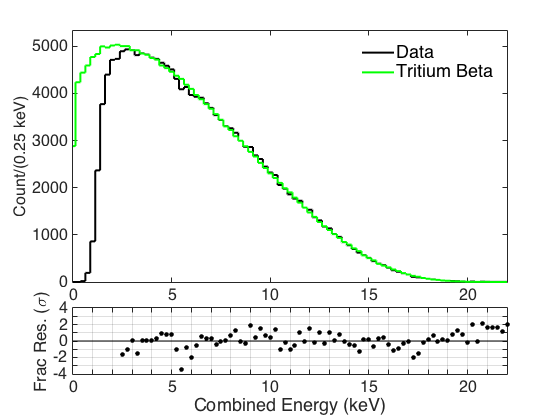
\includegraphics[width=90mm]{fig/tritium-spectrum-linear.png}
\caption{The tritium energy spectrum measured by LUX with the combined energy model (black) compared to several theory models: a pure tritium spectrum (dashed blue), and a tritium spectrum convolved with detector resolution $\rm \frac{\sigma_E}{W} = \sqrt{\sigma_{n_{\gamma_{Det}}}^2 + \sigma_{n_{e_{Det}}}^2}$, described in \cite{Dobi_Thesis}. }
\label{fig:tritium-spectrum}
\end{center}
\end{figure}

%S1 ($\rm \sigma_{n_{\gamma_{Det}}})$ and S2 ($\rm \sigma_{n_{e_{Det}}}$)

A scatter plot of $n_e$ vs $n_{\gamma}$ for the tritium data at 180 V/cm is shown in Fig. \ref{fig:tritium-scatter}, along with the projected histograms on each axis. Contours of constant energy in 1 keV intervals are also plotted, derived from equation \ref{platzman_eq}. Individual events on the plot are smeared by detector resolution and electron-ion pair recombination fluctuations. Detector resolution is comprised of statistical fluctuations in counting photons and electrons in the S1 and S2 channel. The finite resolution in S1 and S2 smear events along the vertical and horizontal axis, respectively. Recombination fluctuations ($\rm \sigma_R$) smear events along the contours of constant energy, and thus cancel out in the combined energy model of Eq.\ref{platzman_eq}. The tritium energy spectrum, obtained by projecting the data along the lines of constant energy, is shown in Fig. \ref{fig:tritium-spectrum}. The data is compared a pure tritium spectrum \cite{Tritium_Eq_Simpson}, with no detector effects, and a tritium spectrum with energy smearing factor of $\rm \frac{\sigma_E}{W} = \sqrt{\sigma_{n_{\gamma_{Det}}}^2 + \sigma_{n_{e_{Det}}}^2}$, described in \cite{Dobi_Thesis}, where $\rm \sigma_{n_{\gamma_{Det}}}$ and $\rm \sigma_{n_{e_{Det}}}$ represent the detector resolution for photon and electron counting. The ratio of the data to the theoretical spectrum is shown in Fig. \ref{fig:ER-threshold}, along with a fit to an error function. The ratio is used to calculate the energy threshold of the detector, the effective 50\% energy threshold is found to be 1.30 $\pm$ 0.013 keV. The good agreement between data and theory to the end of the tritium spectrum demonstrates the linearity of the energy model in Eq.\ref{platzman_eq} down to 2 keV.

\begin{figure}[h!]\centering
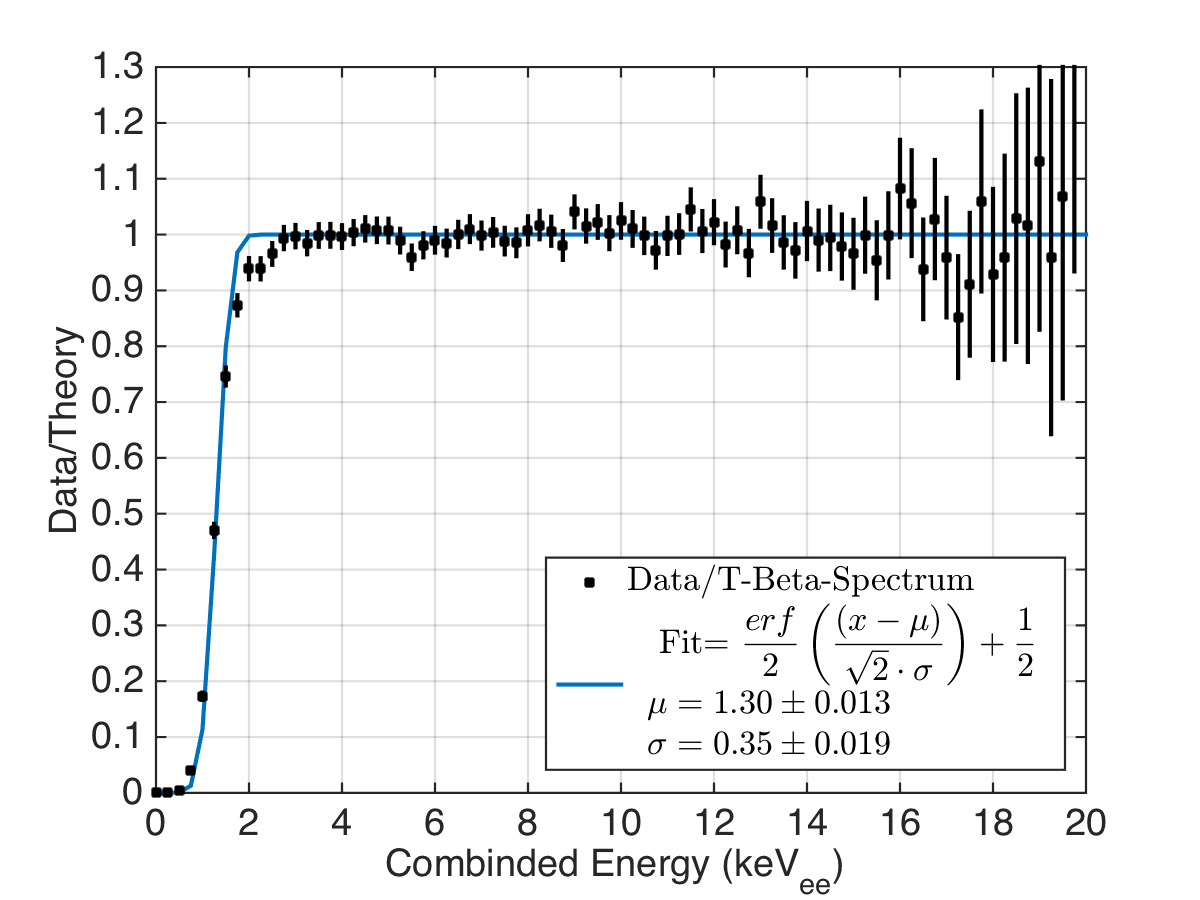
\includegraphics[width=90mm]{fig/E_Thres_Fit.png}
\caption{ER threshold measured by comparing the measured energy spectrum to the smeared tritium spectrum. A fit to an error function is shown.}
\label{fig:ER-threshold}
\end{figure}

The mean light yield and charge yield of ER events in LUX are obtained by dividing the mean light and charge signals by the combined energy in each energy bin. The result is shown for 180 V/cm and 105 V/cm in Fig. \ref{fig:ER-LY-QY} along with NEST model predictions at each field \cite{NEST_2013}. For these plots a small correction has been applied to the data to account for smearing of tritium events across energy bins due to the detector's resolution and the spectral shape \cite{Dobi_Thesis}. 
The light yield results are compared to recent measurements using Compton scatters buy normalizing the signal to the yield of the 32.1 keV decay of $\rm ^{83m}Kr$ at zero field, shown in Fig. \ref{fig:Re_LY}. The light yield of the 32.1 keV decay of $\rm ^{83m}Kr$ at zero field was measured in LUX to be 63.8 +/- 3 $n_\gamma$/KeV.  The findings are consistent with the expectation that tritium light yield data at 100 and 180 V/cm lie between the zero field and 450 V/cm light yield measurements from \cite{Aprile_LY} and \cite{Baudis}. This provides a crucial cross check that the ER band calibration using the tritium beta source is valid for use with the more generic backgrounds found in WIMP search data consisting of Compton scatter from high energy gammas. Compton scatters comprises about 2/3 of the expected background in LUX with the remaining 1/3 being from the beta decay of $\rm ^{85}Kr$ \cite{LUX_BG}. At low energies betas and gammas leave similar track lengths and produce identical yields \cite{NEST} \cite{NEST_2013}. 

Another potential systematic with the tritiated methane calibration is the methane concentration in the xenon. Quenching of light yield from methane is only noticeable at $\sim$ \% level concentrations \cite{Kirill_Methane}. For the work shown here there was less than 1 part per trillion ($<$ $\rm10\times10^{-12}$ g/g) of methane mixed with the xenon. We have verified by using an internal $^{83m}Kr$ calibration source that even 1 part per million of methane is too small quench light yield in liquid xenon \cite{Dobi_Thesis}.


\begin{figure}[h!]\centering
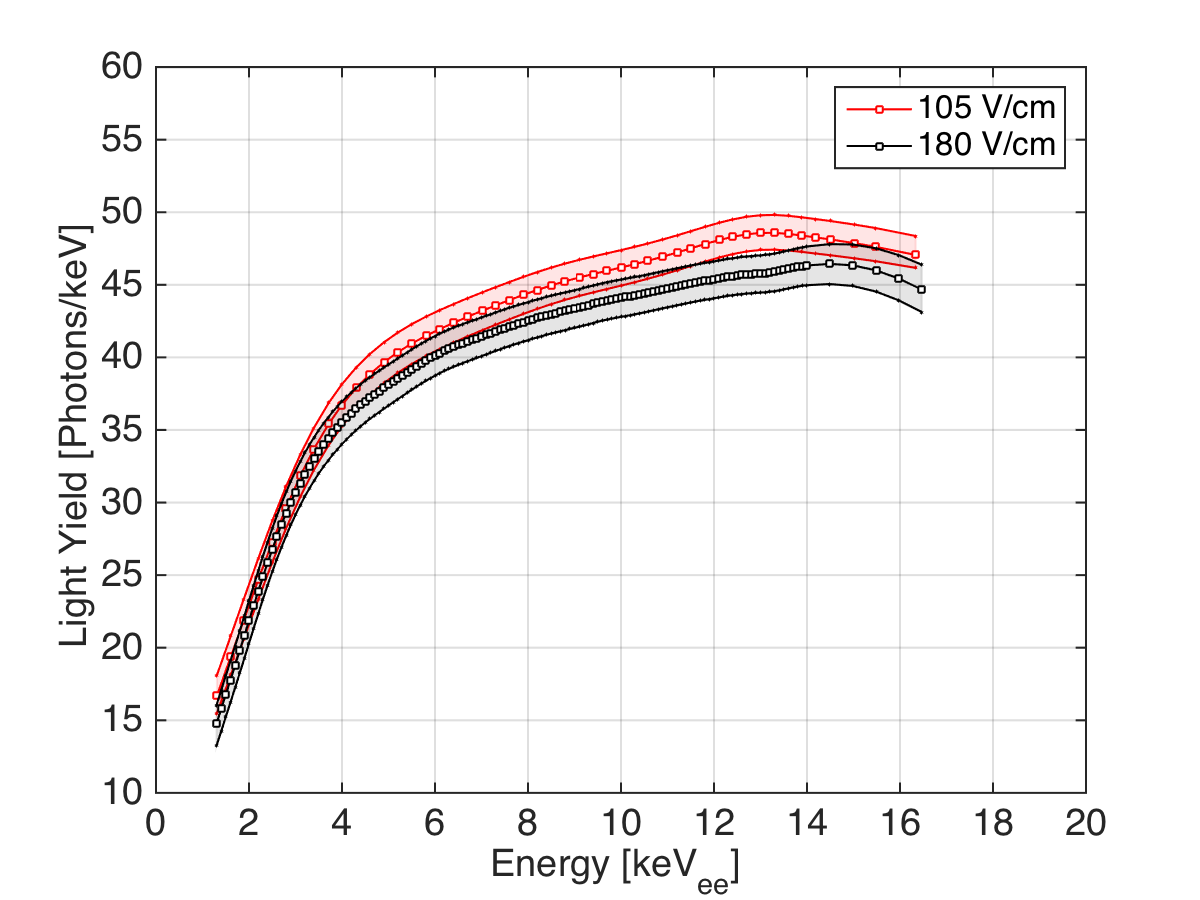
\includegraphics[width=90mm]{fig/ER_LY.png}
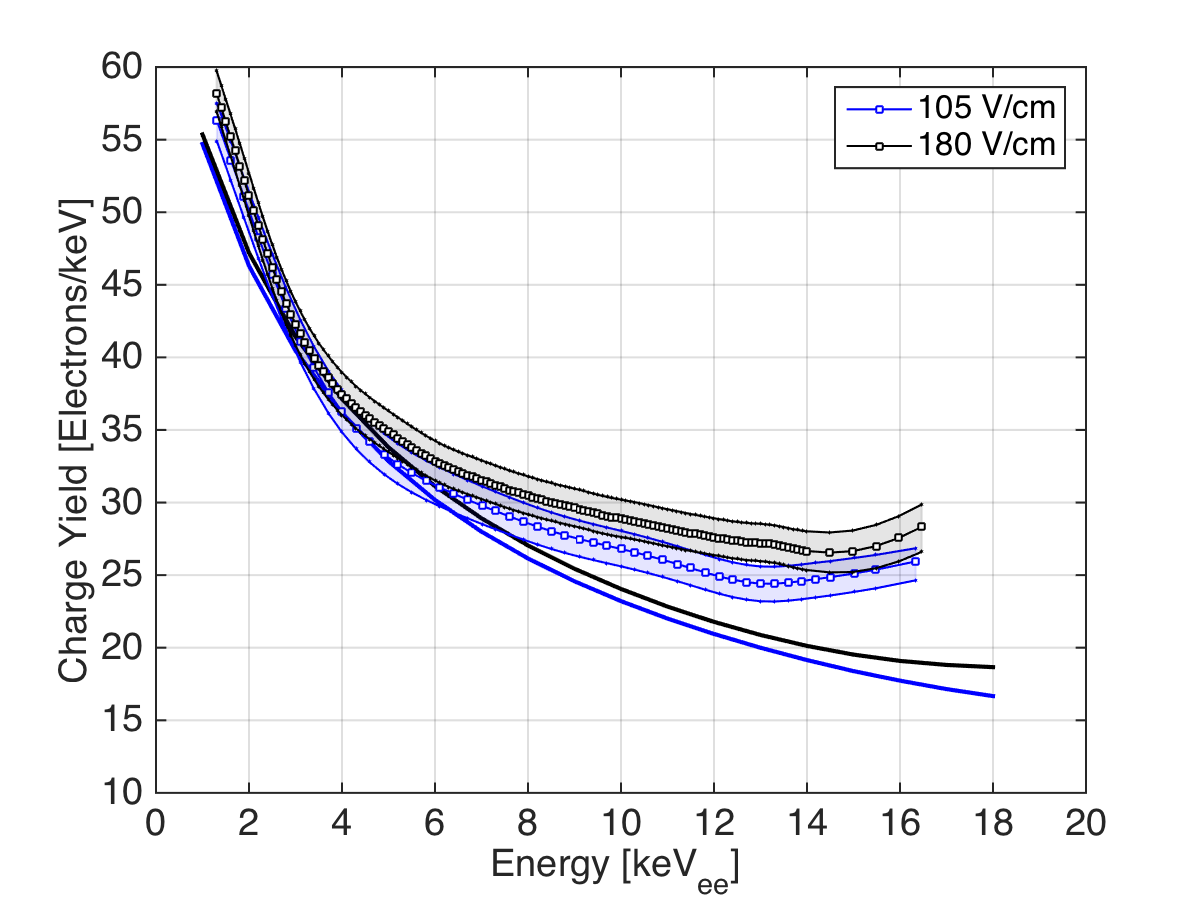
\includegraphics[width=90mm]{fig/ER_QY.png}
\caption{The light yield and charge yield of ER events in LUX at 180 V/cm (black) and 105 V/cm (blue) compared to NEST v0.98 (2013). The bands indicate the systematic errors on $g_1$ and $g_2$, which are fully correlated across all energy bins. $g_1$ is anti-correlated with $g_2$, such that an increase in the charge yield within the grey band must be compensated by an equivalent decrease in the light yield. Upper: Light yield. Lower: the charge yield. The solid lines represent the NEST model predictions at each field \cite{NEST_2013}.}
\label{fig:ER-LY-QY}
\end{figure}

 \begin{figure}[h!]\centering
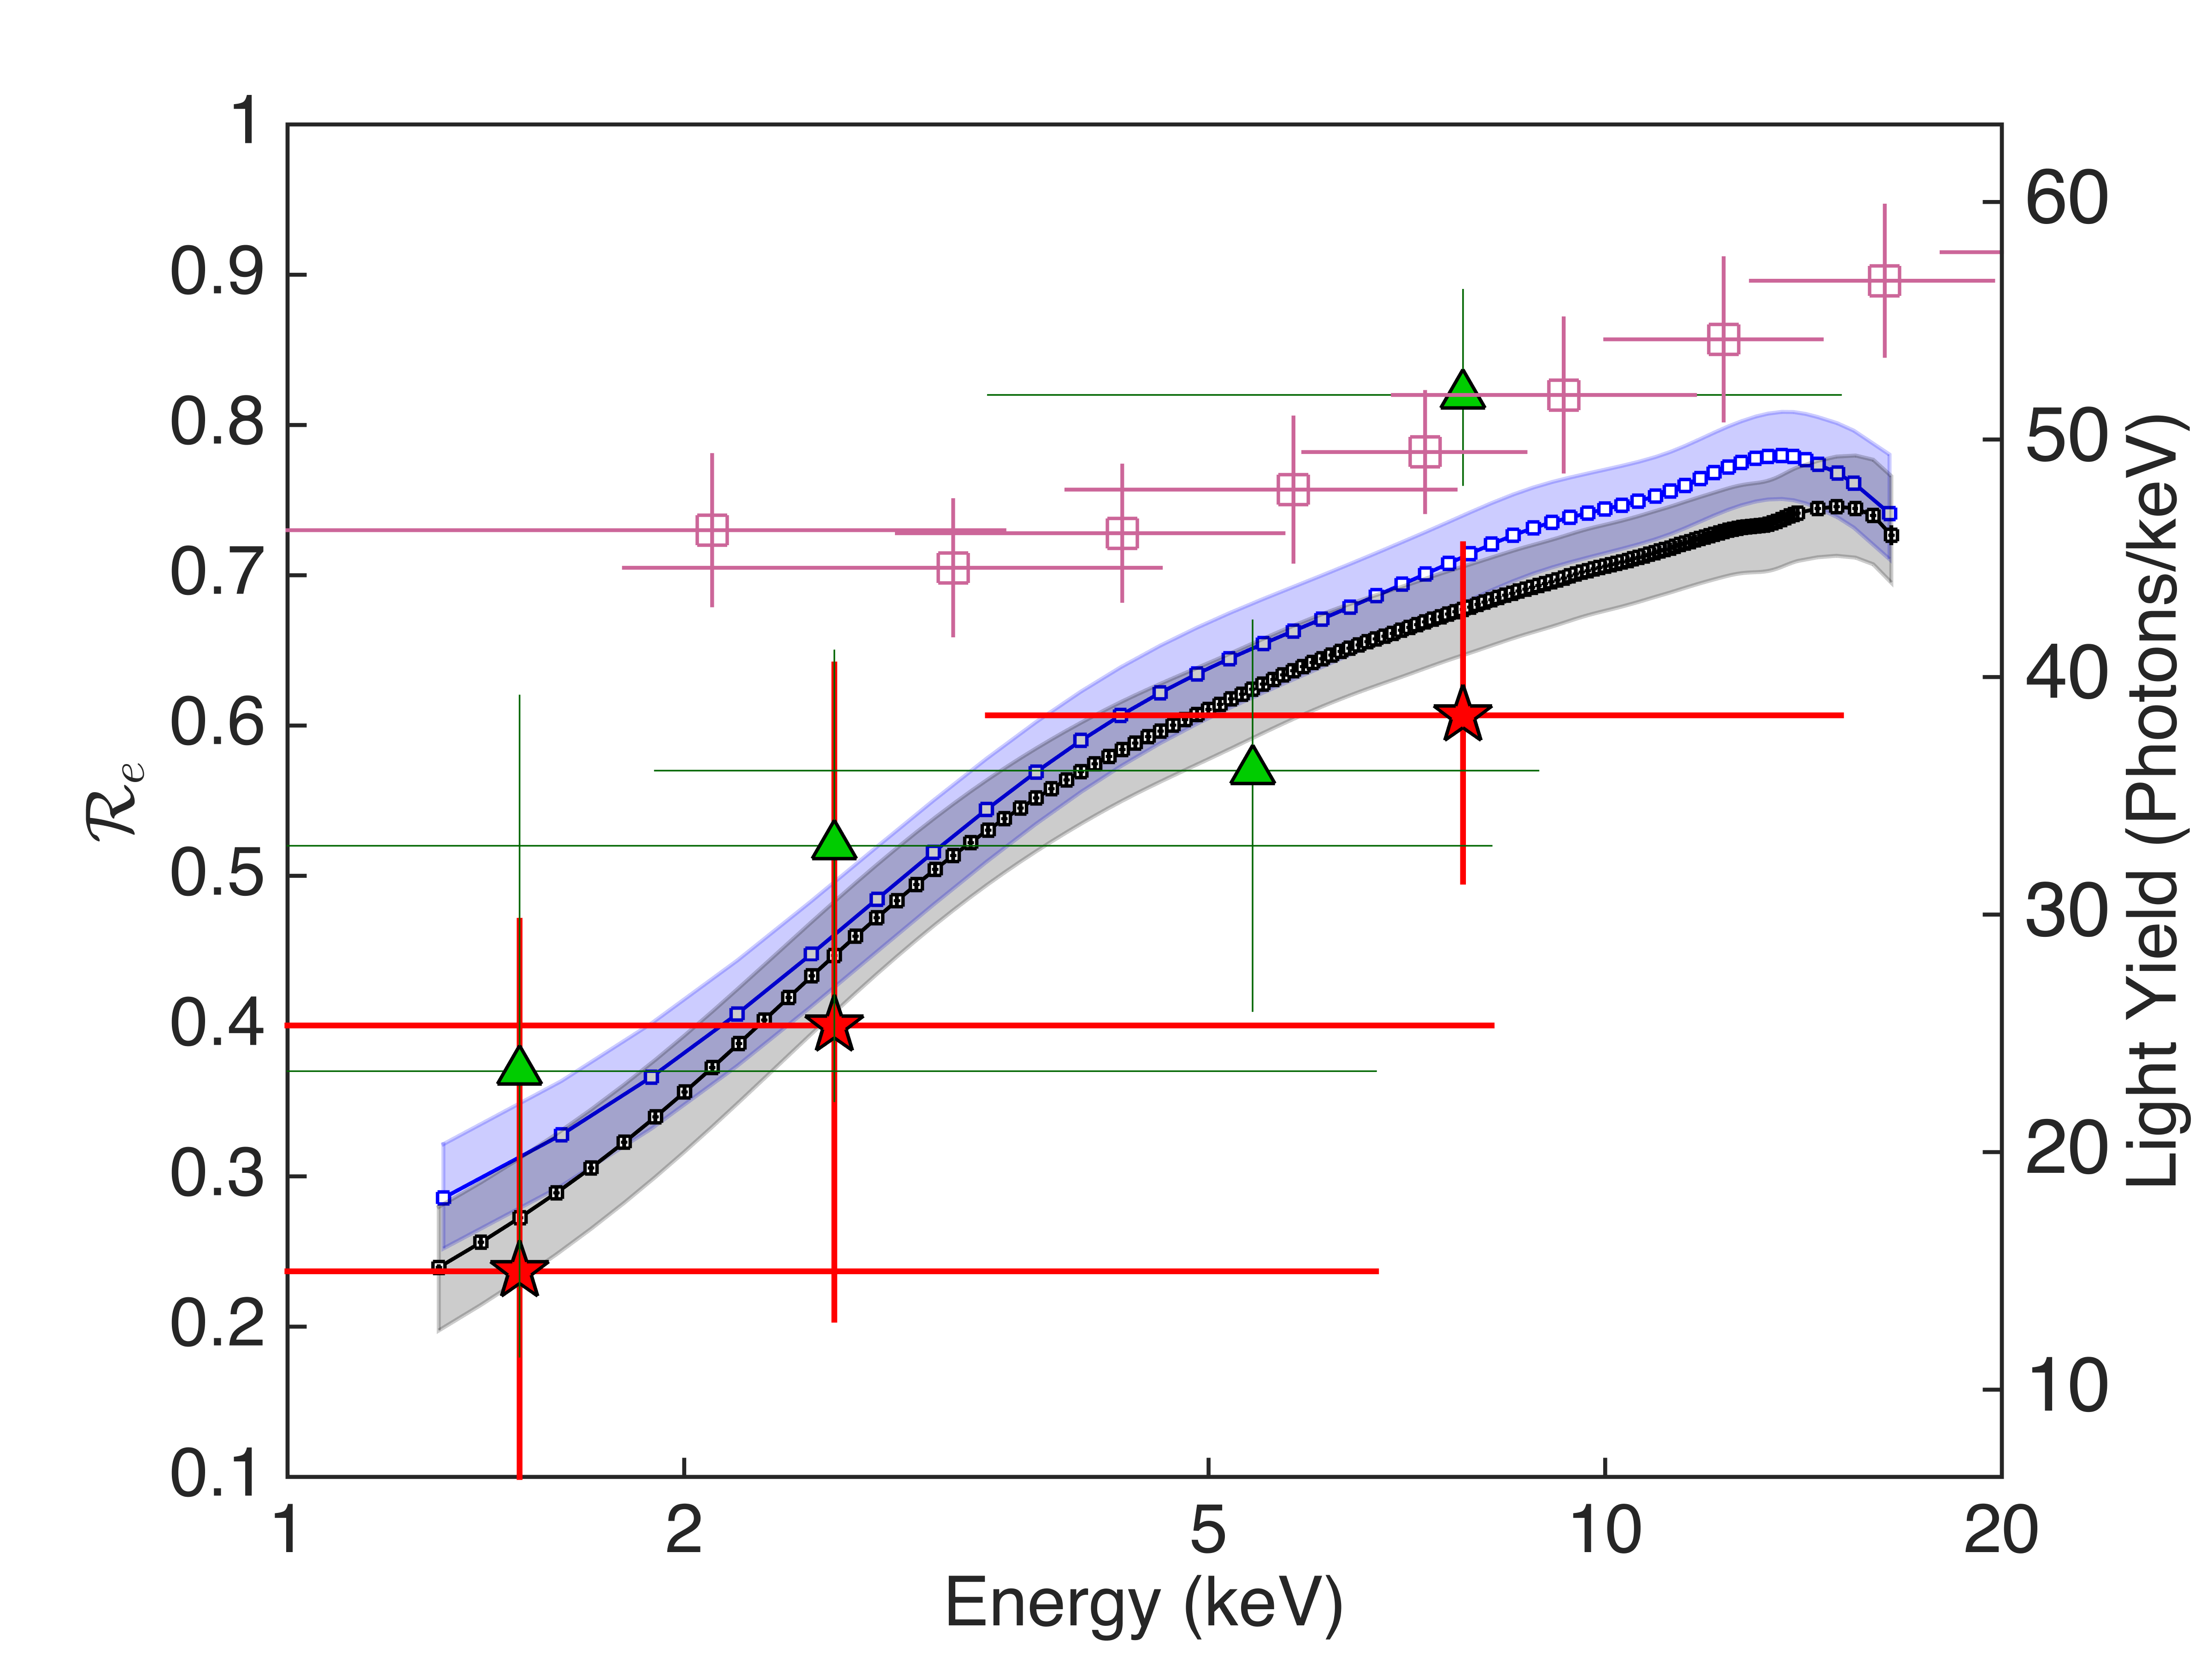
\includegraphics[width=88mm]{fig/Re_LY_log.png}
\caption{Light yield relative to the light yield of the 32.1 keV decay of $\rm^{83}Kr $ at zero field. Shaded blue curve is tritium at 105 [V/cm], shaded black curve is tritium at 180 [V/cm], red circles represent a recent Compton scattering measurement at zero field and 450 [V/cm]. }
\label{fig:Re_LY}
\end{figure}


As shown in Fig. \ref{fig:ER-LY-QY}, the light yield is observed to increase rapidly from 1 and 6 keV, and then becomes mostly energy independent over the remainder of the tritium spectrum. The charge yield exhibits the complimentary behavior as the sum of the two is a constant equal to $\rm \frac{1}{W}=73$. These effects can also be illustrated by plotting the total number of quanta (photons and electrons or excitons and ions) as a function of energy, as shown in Fig. \ref{fig:quanta-vs-energy}. Also shown in Fig. \ref{fig:quanta-vs-energy} are the total number of quanta assuming a $W$ value of 13.7 eV/quanta (black), and the primary number of ions (violet) and excitons (cyan) prior to recombination assuming an initial exciton-to-ion ratio of 0.2 \cite{alpha-value}. We interpret the charge yield data as a measure the recombination fraction at each energy according to

\begin{displaymath}
r = \frac{\frac{n_{\gamma}}{n_e} - \alpha}{\frac{n_{\gamma}}{n_e} + 1}
\end{displaymath}

\noindent
where $r$ is the recombination fraction and $\alpha$ is the initial exciton-to-ion ratio. The recombination fraction as a function of energy as shown in Fig. \ref{fig:recombination}. Here the falling charge yield and rising light yield between 1 and 6 keV appears as a rapid rise in the recombination fraction. 


\begin{figure}[h!]\centering
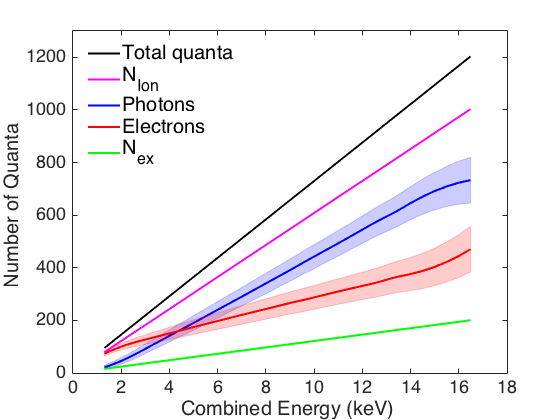
\includegraphics[width=90mm]{fig/quanta-vs-energy.png}
\caption{The mean number of electrons (red) and scintillation photons (blue) produced in LUX at 180 V/cm as a function of energy. The bands indicate the correlated systematic errors on $g_1$ and $g_2$. Also shown are the total number of quanta, primary ions, and primary excitons, assuming an exciton to ion ratio of 0.2. }
\label{fig:quanta-vs-energy}
\end{figure}


\begin{figure}[h!]\centering
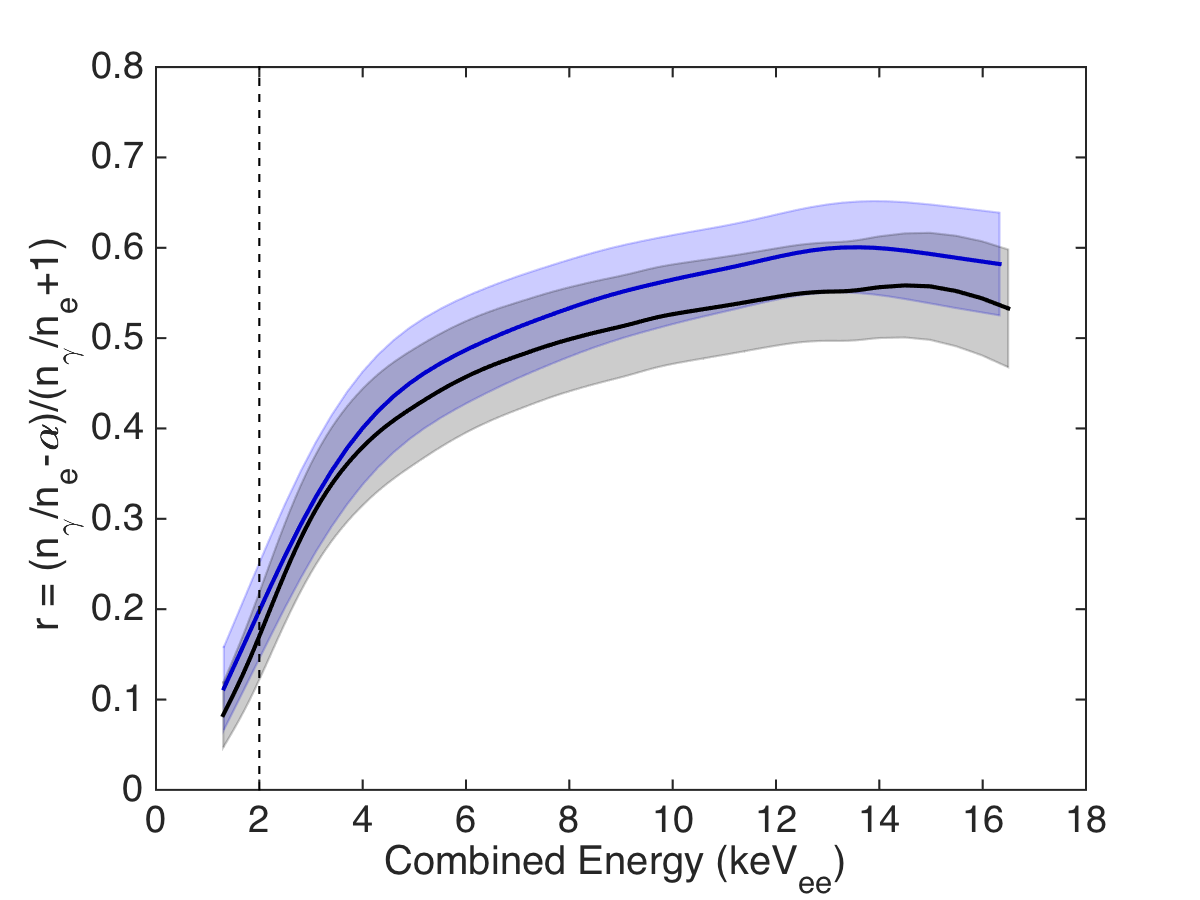
\includegraphics[width=90mm]{fig/recombination.png}
\caption{Recombination fraction of ER events at 180 V/cm (black) and 105 V/cm (blue), assuming an exciton-to-ion ratio of 0.2.}
\label{fig:recombination}
\end{figure}

Having measured the light and charge yield in-situ we have an understanding of the mean of the electron recoil population for the LUX the WIMP search. To complete the picture we need to understand the variance that lead to the width of the electron recoil band. This is comprise of detector resolution, which is measurable and specific to each detector, and recombination fluctuations. At a given energy the event-to-event standard deviation for the number of recombined ions $\rm \sigma_R$ is shown in Fig. \ref{fig:recomb-flucs}, extracted using a method outlined in \cite{Dobi_Thesis}. $\rm \sigma_R$ is a physical property of xenon and produces and irreducible width to the electron recoil band, even with infinite detector resolution. Currently no models exist to predict recombination fluctuations ($\rm \sigma_R$), thus it is important to measure it in-situ. For the LUX detector conditions we find a linear growth in recombination fluctuations as a function of the number of ions $\rm \sigma_R = (0.062 \pm 0.005)\cdot N_{ions}$, consistent with the measurement in \cite{Dobi_Thesis}.

\begin{figure}[h!]\centering
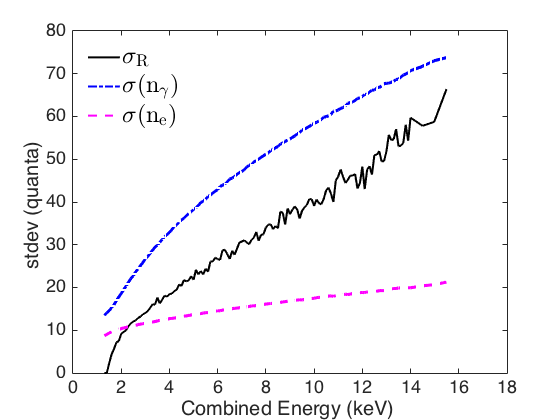
\includegraphics[width=90mm]{fig/recomb_flucs.png}
\caption{Black: recombination fluctuations extracted by a method described in \cite{Dobi_Thesis}. Dot-dash blue: Detector resolution for counting photons. Dashed magenta: Detector resolution for counting electrons. The efficiency for detecting events falls below 95\% below 2 $\rm keV_{ee}$.}
\label{fig:recomb-flucs}
\end{figure}

We obtain the LUX ER band by plotting log$_{10}$(S2/S1) vs S1 as shown in Fig. \ref{fig:ER_band}, this is analogous to plotting the ratio of the charge-to-light ratio vs S1. Also shown is the LUX NR band measured with DD neutron generator data. The ER band has a characteristic rise at low S1 which reflects the increasing charge yield and decreasing light yield below 4 keVee, as seen in Fig. \ref{fig:quanta-vs-energy}. The leakage fraction ($f$), defined as the fraction of ER events that fall below the mean of the NR band, is shown in Fig. \ref{fig:Leak} as a function of S1. The recoil discrimination ($1-f$) has an average value of \fixit{99.8\%} for events with S1 between 1 and 50 phd.

\begin{figure}[h!]\centering
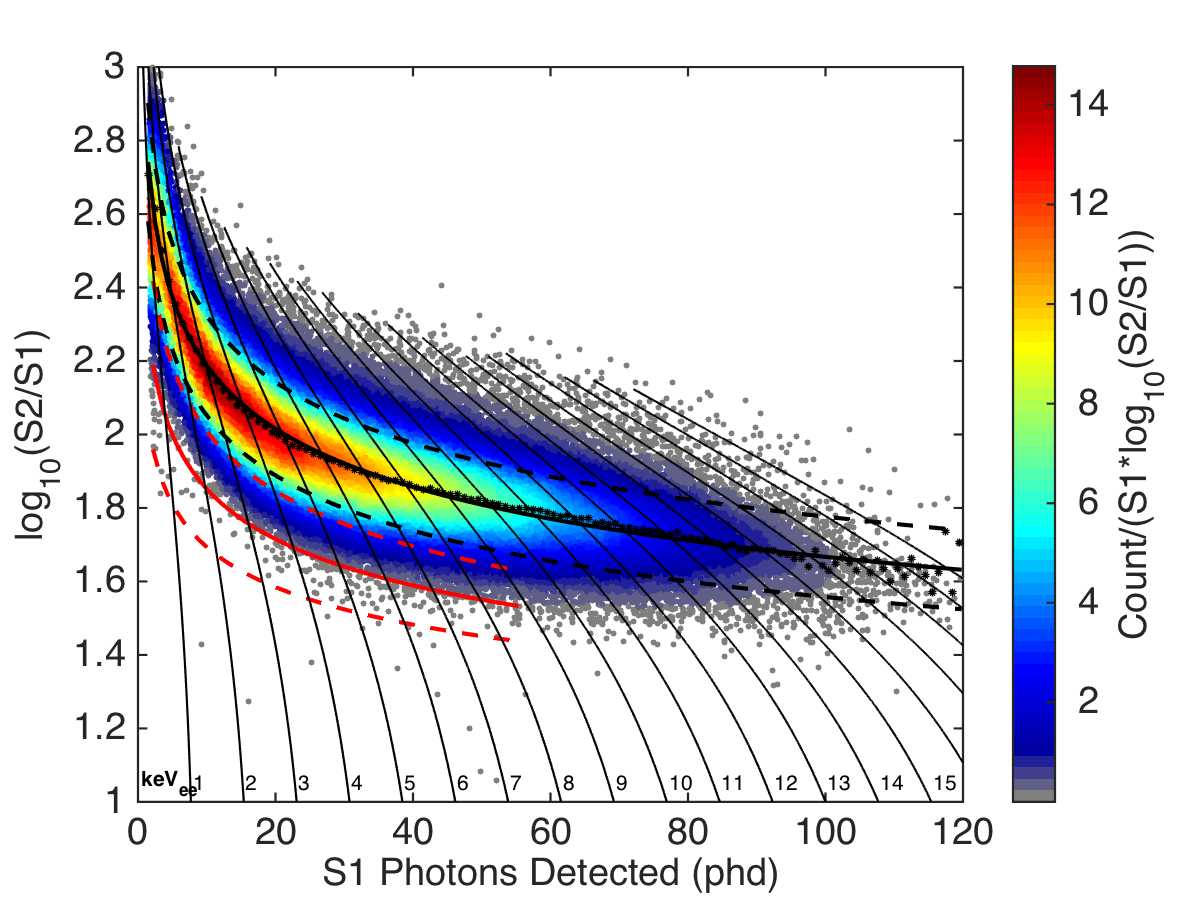
\includegraphics[width=100mm]{fig/CH3T_ER_Band.png}
\caption{The electron recoil band of LUX illuminated by 130,000 tritium events at the nominal LUX electric field of 180 V/cm.  The recoil discriminant variable, log(S2/S1), is shown vs. S1 between 1 and 50 phd in S1 (about $\rm1-8 keV_{ee}$). Also indicated in black are the mean and the 10\% and 90\% contours. The solid red line represents the mean NR band determined with DD neutron generator data. The dashed red indicates the 10\% and 90\% contours of the NR band.}
\label{fig:ER_band}
\end{figure}

\begin{figure}[h!]\centering
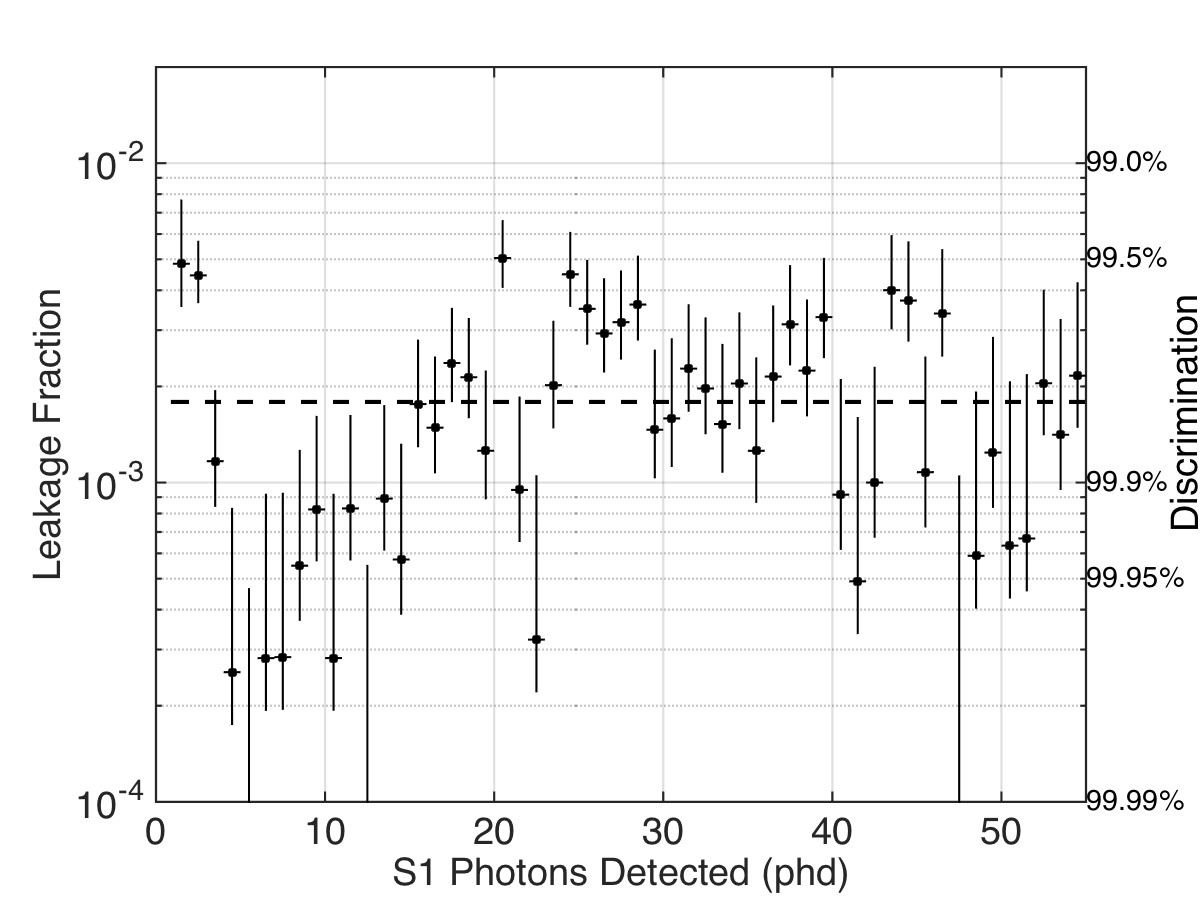
\includegraphics[width=90mm]{fig/CH3T_Leakage_Run03.png}
\caption{LUX recoil discrimination vs. S1, determined from Fig. \ref{fig:ER_band}. Y-axis labels: left -  leakage fraction ($f$); right - discrimination ($1-f$).}
\label{fig:Leak}
\end{figure}


%% ER band Gaussianity section. If we want this

Using the high statistics tritium data along with knowing the data purity of 4 non tritium ER events out of 180,000 in the fiducial the ER band Gaussianity is characterized. Experiments in the past have relied on the assumption that the bands can be modeled with a log-normal distribution using the discrimination variable $\rm log_{10}(S2/S1)$ vs. S1. It is found that this assumption holds to roughly 3 sigma out past which events are observed out to 8 sigma with a constant likelihood of $\sim$ 1/100,000 which corresponds to  roughly 4 sigma. This is a crucial piece of information that allows us to build a pdf for the ER events, as events out at several sigma may be assigned an incorrect likelihood using a Gaussian model. Fig. \ref{fig:ER-Gauss} shows the ER event distribution in 3 phd bins of S1 for the centroid subtracted $\rm log_{10}(S2/S1)$ population.


%\onecolumngrid
\begin{sidewaysfigure}[p!]\centering
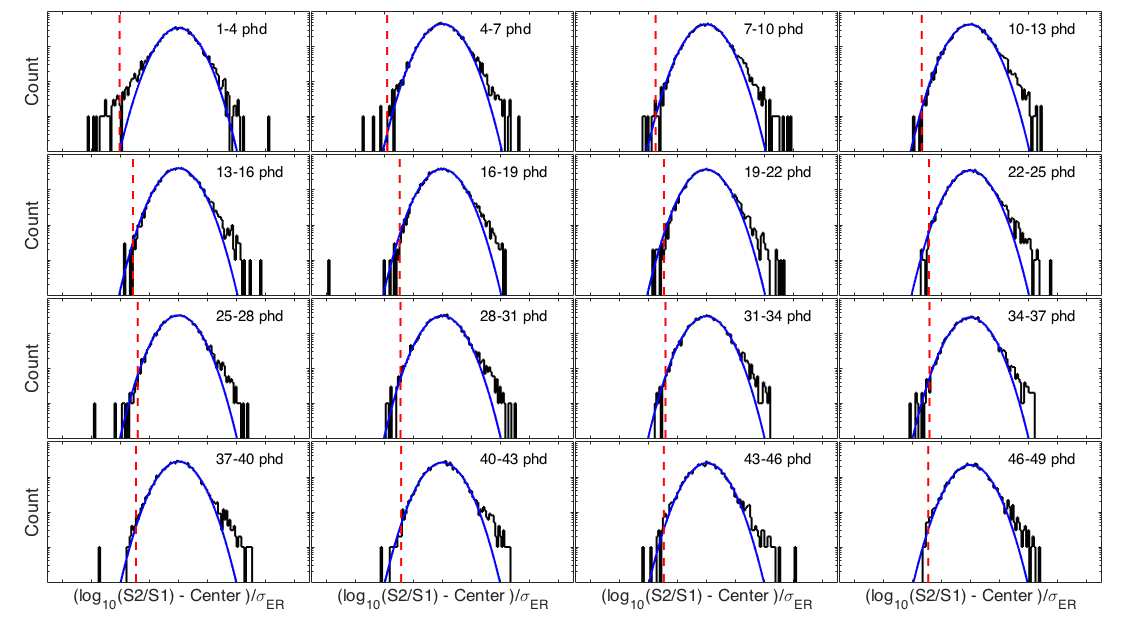
\includegraphics[width=150mm]{fig/Gaussianity/GaussER_all.png}
\caption{}
\label{fig:ER-Gauss}
\end{sidewaysfigure}
%\twocolumn

Using the information obtained from the tritium calibration source we can fully characterize the electron recoil band for the LUX WIMP search. The mean light and charge yield measure the mean location of the electron recoil population and the variance arrises from detector resolution convolved with recombination fluctuations. The tritium calibration allows for a detailed measure of the underlying properties of electron recoils and thus an improves background modeling for any dark matter experiment.
%%%%%%%%%%%%%%%%%%%%%%%%%%%%%%%%%%%%%%%%%%%%%%%%%%%%%%%%%%

